\Chapter{Applications}
\label{chap:applications}

\Section{Remote access}

\Paragraph{Telnet}
\mode<article>{
Telnet is an application protocol used on a network to provide a bidirectional interactive text-oriented communication facility using a virtual terminal connection.
Telnet was developed in 1969.
The name stands for `teletype network.'

Historically, Telnet provided access to a command-line interface on a remote host.
However, because of serious security concerns -- it sends all data, including passwords, in clear-text over the network -- when using Telnet over an open network such as the internet, its use for this purpose has waned significantly in favour of \acs{SSH}.
}

\Paragraph{\acs{SSH}}
\mode<article>{
The \acf{SSH} protocol is a cryptographic network protocol for operating network services securely over an unsecured network.
Its most notable applications are remote login and command-line execution.

\acs{SSH} was first designed in 1995.
The most commonly implemented software stack is OpenSSH, released in 1999 as open-source software by the OpenBSD developers.
Implementations are distributed for all types of operating systems in common use, including embedded systems.
In Windows 10 version 1709, an official Win32 port of OpenSSH is available.
}

\Section{File transfer}

\Paragraph{\acs{FTP}}
\mode<article>{
The \acf{FTP} is a standard communication protocol used for the transfer of computer files from a server to a client on a computer network.
\acs{FTP} is built on a client–server model architecture using separate control and data connections between the client and the server.
\acs{FTP} users may authenticate themselves with a clear-text sign-in protocol, normally in the form of a username and password, but can connect anonymously if the server is configured to allow it.
}

\Paragraph{active vs passive}
\mode<article>{
\acs{FTP} may run in active or passive mode, which determines how the data connection is established.
In active mode, the client starts listening for incoming data connections from the server on port $M$.
It sends the \acs{FTP} command \abbr{PORT M} to inform the server on which port it is listening.
The server then initiates a data channel to the client from its port~20, the \acs{FTP} server data port.

In situations where the client is behind a firewall and unable to accept incoming \acs{TCP} connections, passive mode may be used.
In this mode, the client uses the control connection to send a \abbr{PASV} command to the server and then receives a server \acs{IP} address and server port number from the server, which the client then uses to open a data connection from an arbitrary client port to the server \acs{IP} address and server port number received.
}

\Paragraph{\acs{TFTP}}
\mode<article>{
\acf{TFTP} is a simple file transfer protocol which allows a client to get a file from or put a file onto a remote host.
One of its primary uses is in the early stages of nodes booting from a local-area network.
\acs{TFTP} has been used for this application because it is very simple to implement.

Due to its simple design, \acs{TFTP} can be easily implemented by code with a small memory footprint.
It is therefore the protocol of choice for the initial stages of any network booting strategy like \acs{BOOTP}, \acs{PXE}, \acs{BSDP}, etc., when targeting from highly resourced computers to very low resourced \ac{SBC} and \ac{SOC}.
It is also used to transfer firmware images and configuration files to network appliances like routers, firewalls, \acs{IP} phones, etc.
}

\Paragraph{\acs{FTPS}}
\mode<article>{
\ac{FTPS} (also known \acs{FTP}-\acs{SSL}) is an extension to the commonly used \acf{FTP} that adds support for the \acf{TLS} and, formerly, the \acf{SSL} cryptographic protocols.

Because \acs{FTP} uses a dynamic secondary port (for data channels), many firewalls were designed to snoop \acs{FTP} control messages in order to determine which secondary data connections they need to allow.
However, if the \acs{FTP} control connection is encrypted using \acs{TLS}/\acs{SSL}, the firewall cannot determine the \acs{TCP} port number of a data connection negotiated between the client and \acs{FTP} server.
Therefore, in many firewalled networks, an \acs{FTPS} deployment will fail when an unencrypted \acs{FTP} deployment will work.
This problem can be solved with the use of a limited range of ports for data and configuring the firewall to open these ports.
}

\Paragraph{\acs{SFTP}}
\mode<article>{
The \acl{SFTP} is a network protocol that provides file access, file transfer, and file management over any reliable data stream.
It was designed by the \acs{IETF} as an extension of the \acf{SSH} protocol version~2.0 to provide secure file transfer capabilities.

This protocol assumes that it is run over a secure channel, such as \acs{SSH}, that the server has already authenticated the client, and that the identity of the client user is available to the protocol.

\acs{SFTP} is not \acs{FTP} run over \acs{SSH}, but rather a new protocol designed from the ground up by the \acs{IETF} \abbr{SECSH} working group.
}

\Section{\acl{DNS}}

\mode<article>{
The \acf{DNS} is the hierarchical and decentralised naming system used to identify computers reachable through the internet or other \acs{IP} networks.
The resource records contained in the \acs{DNS} associate domain names with other forms of information.
These are most commonly used to map human-friendly domain names to the numerical \acs{IP} addresses computers need to locate services and devices using the underlying network protocols, but have been extended over time to perform many other functions as well.
The \acl{DNS} has been an essential component of the functionality of the internet since 1985.
}

\Paragraph{authoritative server}
\mode<article>{
An authoritative name server is a name server that only gives answers to \acs{DNS} queries from data that has been configured by an original source, for example, the domain administrator or by dynamic \acs{DNS} methods, in contrast to answers obtained via a query to another name server that only maintains a cache of data.
}

\Paragraph{resolver}
\mode<article>{
The client side of the \acs{DNS} is called a \acs{DNS} resolver.
A resolver is responsible for initiating and sequencing the queries that ultimately lead to a full resolution (translation) of the resource sought, e.g., translation of a domain name into an \acs{IP} address.
\acs{DNS} resolvers are classified by a variety of query methods, such as \emph{recursive}, \emph{non-recursive}, and \emph{iterative}.
A resolution process may use a combination of these methods.

In a \emph{non-recursive} query, a \acs{DNS} resolver queries a \acs{DNS} server that provides a record either for which the server is authoritative, or it provides a partial result without querying other servers.

In a \emph{recursive} query, a \acs{DNS} resolver queries a single \acs{DNS} server, which may in turn query other \acs{DNS} servers on behalf of the requester.
For example, a simple stub resolver running on a home router typically makes a recursive query to the \acs{DNS} server run by the user's \acs{ISP}.
A recursive query is one for which the \acs{DNS} server answers the query completely by querying other name servers as needed.

The \emph{iterative} query procedure is a process in which a \acs{DNS} resolver queries a chain of one or more \acs{DNS} servers.
Each server refers the client to the next server in the chain, until the current server can fully resolve the request.
For example, a possible resolution of www.ex\-am\-ple.com would query a global root server, then a `com' server, and finally an `example.com' server.
}

\Paragraph{address resolution}
\mode<article>{
The process of address resolution is shown in \vref{fig:dns}.
The computer in the top left corner wants to acccess the server `example.com.'
The client computer queries its local \acs{DNS} resolver using a recursive query (step~1) for the \acs{IP} address of example.com.
The resolver uses iterative queries to retrieve the required \acs{IP} address (steps~2 through 7).
After the client receives the \acs{IP} address from the resolver (step~8) it can initiate communication with the server (steps~9 and~10).


\begin{figure}
\centering
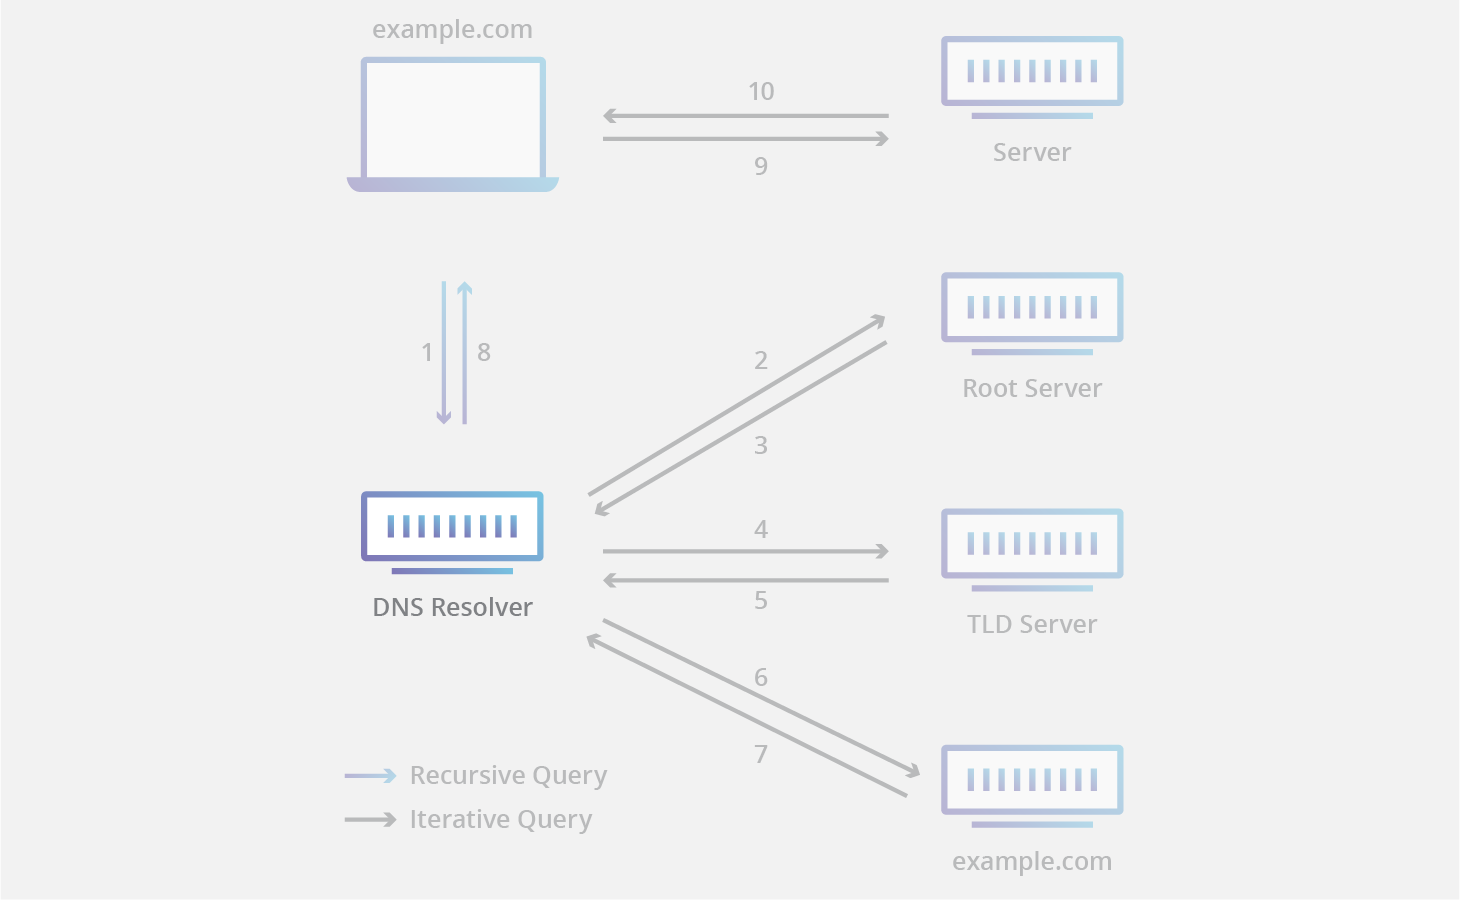
\includegraphics[width=\textwidth]{images/recursive-resolver.png}
\caption{\acs{DNS} address resolution}
\label{fig:dns}
\end{figure}

}

\Paragraph{\acs{mDNS}}
\mode<article>{
When a \acl{mDNS} client needs to resolve a hostname, it sends an \acs{IP} multicast query message that asks the host having that name to identify itself.
That target machine then multicasts a message that includes its \acs{IP} address.
All machines in that subnet can then use that information to update their \acs{mDNS} caches.
Any host can relinquish its claim to a name by sending a response packet with a \acf{TTL} equal to zero.

By default, \acs{mDNS} exclusively resolves hostnames ending with the `.local' top-level domain.
This can cause problems if .local includes hosts that do not implement \acs{mDNS} but that can be found via a conventional unicast \acs{DNS} server.
Resolving such conflicts requires network configuration changes that \acs{mDNS} was designed to avoid.
}

\Section{Email}

\mode<article>{
Email operates across computer networks, primarily the internet, and also local-area networks.
Today's email systems are based on a store-and-forward model.
Email servers accept, forward, deliver, and store messages.
Neither the users nor their computers are required to be online simultaneously; they need to connect, typically to a mail server or a webmail interface to send or receive messages or download it.
}

\Paragraph{\acs{SMTP}}
\mode<article>{
The \acl{SMTP} is an internet standard communication protocol for electronic mail transmission.
Mail servers and other message transfer agents use \acs{SMTP} to send and receive mail messages.
User-level email clients typically use \acs{SMTP} only for sending messages to a mail server for relaying, and typically submit outgoing email to the mail server on port~587 or~465 per \rfc{8314}.

\acs{SMTP} servers commonly use the \acf{TCP} on port number~25 (for plaintext) and~587 (for encrypted communications).
}

\Paragraph{\acs{POP3}}
\mode<article>{
The \acl{POP3} provides access via an \acs{IP} network for a user client application to a mailbox (\emph{maildrop}) maintained on a mail server.
The protocol supports download and delete operations for messages.
\acs{POP3} clients connect, retrieve all messages, store them on the client computer, and finally delete them from the server.
This design of \acs{POP3} and its procedures was driven by the need of users having only temporary internet connections, such as dial-up access, allowing these users to retrieve email when connected, and subsequently to view and manipulate the retrieved messages when offline.

A \acs{POP3} server listens on well-known port number~110 for service requests.
Encrypted communication for \acs{POP3} is either requested after protocol initiation, using the \abbr{STLS} command, if supported, or by \acs{POP3S}, which connects to the server using \acs{TLS} or \acs{SSL} on well-known \acs{TCP} port number~995.
}

\Paragraph{\acs{IMAP}}
\mode<article>{
The \acl{IMAP} was designed with the goal of permitting complete management of an email box by multiple email clients, therefore clients generally leave messages on the server until the user explicitly deletes them.
An \acs{IMAP} server typically listens on port number~143.
\acs{IMAP} over \acs{SSL}/\acs{TLS} (\acs{IMAPS}) is assigned the port number~993.
}

\Paragraph{webmail}
\mode<article>{
Companies no longer host their own email servers using Postfix or Microsoft Exchange.
Instead they use cloud solutions like Gmail or Office~365.
}

\Paragraph{spam}
\mode<article>{
Email spam has steadily grown since the early 1990s, and by 2014 was estimated to account for around ninety percent of total email traffic.
}

\mode<article>{
\section{Further reading}
\textcite{nemeth} explains all applications and protocols covered in this chapter in more detail and provides the details of how to setup name servers and mail servers.
Some interesting reads are \rfc{1912} and \rfc{2822}.
}